\documentclass[11pt,twoside]{article}
\usepackage{subcaption}
\usepackage{graphicx}
\usepackage{float}
\usepackage{tikz}
\usepackage{calc}
\usepackage{float}
\usepackage{array}
\usepackage{hyperref}

\usepackage{framed}
\usepackage{amsthm}

\newcommand{\HW}{}
\newcommand{\HWnumb}{3}
\newcommand{\HWdate}{Wednesday May 2}
\usepackage{amsmath,amssymb}
\usepackage{url}

\textheight      9.0in
\textwidth       5.5in
\topmargin      -0.1in
\oddsidemargin   0.5in
\evensidemargin  0.5in
\pagestyle{myheadings}

\markboth{MS\&E 318 (CME 338) \quad Large-Scale Numerical Optimization}
         {Spring 2018, Homework \HWnumb}


%% These are some special commands not provided by macros.tex

\newcommand{\problem}[4]{\fbox
   {\begin{tabular*}{0.84\textwidth}
    {@{}l@{\extracolsep{\fill}}l@{\extracolsep{6pt}}%
        l@{\extracolsep{\fill}}c@{}}
      #1 & $\minimize{#2}$ & $#3$ & $ $ \\[5pt]
         & $\subject$      & $#4$ & $ $
    \end{tabular*}}}

\newcommand{\AI}      {(A\ -\!\!I\,)}
\newcommand{\BS}      {\pmat{B & S}}
\newcommand{\BN}      {\pmat{B & N}}
\newcommand{\codes}[1]{$ $\\ \hbox to 0.4\textwidth{#1\hss}}
\newcommand{\Eq}      {&\!=\!&}
\newcommand{\factol}  {\hbox{\tt FacTol}}
%\newcommand{\Matlab}  {{\sc Matlab}}
%\newcommand{\m}       {\phantom-}
\newcommand{\NL}      {_{\scriptscriptstyle N\!L}}
\newcommand{\phibar}  {{\bar\phi}}
\newcommand{\Tab}     {\\ \hspace*{\parindent}}
\newcommand{\To}      {\,{:}\,}  % $p \To q$ gives p:q with proper spacing
\newcommand{\updatetol}{\hbox{\tt UpdateTol}}
\newcommand{\myvec}[2]{{\displaystyle \pmat{#1\\#2}}}
\newcommand{\xs}      {\myvec xs}
\newcommand{\z}       {\phantom 0}

\begin{document}

\thispagestyle{plain}
\begin{center}
           $ $
\\[-0.7in] {\large Stanford University,
                   Management Science and Engineering (and ICME)}
\\[4pt]    {\Large MS\&E 318 (CME 338) \quad  Large-Scale Numerical Optimization}
\\[6pt]    {\large Student: Adele Kuzmiakova \qquad Spring 2018}
\\[7pt]    {\large Homework \HWnumb, Due \HWdate}
\\         {       \url{http://stanford.edu/class/msande318/homework.html}}
\end{center}


%%%%%%%%%%%%%%%%%%
% LaTeX macros.tex
% 27 Apr 2003: \def replaced by \newcommand
% 17 Aug 2005: \Frac fixed (needs {} around #1 and #2).
%              \Newcommand, \pmat, \bmat  introduced.
%              NB: \Newcommand doesn't work with commands that have [] arguments.
% 05 Sep 2005: Added innerproduct
% 08 Dec 2005: Realized that \providecommand already does what we were
%              trying to do with \Newcommand.
% 11 Dec 2005: Revived \Newcommand to overload commands from other packages.
% 13 Aug 2007: AF changed ``\mathrm'' to ``\operator@font''
%%%%%%%%%%%%%%%%%%

\makeatletter
%\newcommand{\proof{\penalty 25\noindent{\bf Proof.}\nobreak\hskip 1em\ignorespaces}

%\newcommand{\emptybox}{\ \vbox{\hrule\hbox{\vrule height1.3ex\hskip0.8ex\vrule}\hrule}}
\newcommand{\emptybox}{\vbox{\hrule height0.6pt\hbox{\vrule height1.3ex width0.6pt\hskip0.8ex%
   \vrule width0.6pt}\hrule height0.6pt}} % SIAM \endproof

\newcommand{\noproof}{\hspace{.5em}\blackslug}
\newcommand{\m}{\phantom-}
\newcommand{\mm}[1]{\hbox{$#1$}}                 % math mode
\newcommand{\mtx}[2]{\renewcommand{\arraystretch}{1.2}%
      \left(\! \begin{array}{#1}#2\end{array}\! \right)}
% The next two are better than \mtx.
\newcommand{\pmat}[1]{\begin{pmatrix}#1\end{pmatrix}}  % Need \usepackage{amsmath}
\newcommand{\bmat}[1]{\begin{bmatrix}#1\end{bmatrix}}

% Does anyone know how to do this with \newcommand?
\ifx   \innerprod\undefined%
   \def\innerprod(#1,#2){\langle#1,#2\rangle} % Must be called as \innerproduct(A,B)
\fi

%%%%%%%%%%%%%%%%%%%%%%%%%%%%%%%%%%%%%%%%%%%%%%%%%%%%%%%%%%%%%%%%%%%%%%%%%%%%%%%%%%%%
%%% Replace commands defined in other packages%%%%%%%%%%%%%%%%%%%%%%%%%%%%%%%%%%%%%%
\newcommand{\Newcommand}[2]%
   {\ifx#1\undefined \newcommand{#1}{#2} \else \renewcommand{#1}{#2} \fi}
\ifx\mod\undefined
  \newcommand{\mod}[1]{|#1|}
\else
  \renewcommand{\mod}[1]{|#1|}
\fi
\ifx\Range\undefined
  \newcommand{\Range}{\mathop{\operator@font{range}}}
\else
  \renewcommand{\Range}{\mathop{\operator@font{range}}}
\fi
\Newcommand{\Re} {\mathbb{R}}           % Need \usepackage{amssymb}
\Newcommand{\subject} {\hbox{\rm subject to}}           % Need \usepackage{amssymb}

%%%%%%%%%%%%%%%%%%%%%%%%%%%%%%%%%%%%%%%%%%%%%%%%%%%%%%%%%%%%%%%%%%%%%%%%%%%%%%%%%%%%
%%% Commands defined in other packages%%%%%%%%%%%%%%%%%%%%%%%%%%%%%%%%%%%%%%%%%%%%%%
\providecommand{\det}  {\mathop{\operator@font{det}}}
\providecommand{\diag} {\mathop{\operator@font{diag}}}
\providecommand{\dim}  {\mathop{\operator@font{dim}}}
\providecommand{\exp}  {\mathop{\operator@font{exp}}}
\providecommand{\Frac}[2]{{\textstyle{\frac{#1}{#2}}}}
%\providecommand{\mod}[1]{|#1|}
\providecommand{\rank} {\mathop{\operator@font{rank}}}
%\providecommand{\Re}   {\mathbb{R}}           % Need \usepackage{amssymb}
\providecommand{\Co}   {\mathbb{C}}            % Need \usepackage{amssymb}
\providecommand{\vec}  {\mathop{\operator@font{vec}}}

%%%%%%%%%%%%%%%%%%%%%%%%%%%%%%%%%%%%%%%%%%%%%%%%%%%%%%%%%%%%%%%%%%%%%%%%%%%%%%%%%%%%
\newcommand{\st}{:}
\newcommand{\abs}[1]{|#1|}
\newcommand{\argmin}{\mathop{\operator@font{argmin}}}
\newcommand{\argmax}{\mathop{\operator@font{argmax}}}
\newcommand{\conv}{\mathop{\operator@font{conv}}}
\newcommand{\eig}{\mathop{\operator@font{eig}}}
\newcommand{\mv}[1]{\mathtt{#1}}
\newcommand{\mtt}[1]{\mathtt{#1}}
\newcommand{\T}{^T\!}
\newcommand{\Tinv}{^{-T}\!}
\newcommand{\und}[1]{$\underline{\hbox{#1}}$}
\newcommand{\gge}{\succeq}
\newcommand{\twonorm}[1]{\norm{#1}_2}
\newcommand{\onenorm}[1]{\norm{#1}_1}
\newcommand{\infnorm}[1]{\norm{#1}_{\infty}}
\newcommand{\dualnorm}[1]{\norm{#1}_D}
\newcommand{\disp}{\displaystyle}
\newcommand{\super}{\scriptstyle}
\newcommand{\superplus}{^{+}}
\newcommand{\superminus}{^{-}}
\newcommand{\ur}{\mbox{\bf u}}
%\newcommand{\Re}{I\!\!R}
\newcommand{\sgap}{\;}
\newcommand{\mgap}{\;\;}
\newcommand{\bgap}{\;\;\;}
%\newcommand{\subject}{\hbox{\rm subject to}}
\newcommand{\minimize}[1]{{\displaystyle\minim_{#1}}}
\newcommand{\minimizearg}[2]{{\displaystyle\minim_{#1 \in \Re^{#2}}}}
\newcommand{\maximizearg}[2]{{\displaystyle\maxim_{#1 \in \Re^{#2}}}}
\newcommand{\minimizetwoarg}[4]{{\displaystyle\minim_{#1 \in \Re^{#2},%
                                                  #3 \in \Re^{#4}}}}
\newcommand{\maximizetwoarg}[4]{{\displaystyle\maxim_{#1 \in \Re^{#2},%
                                                  #3 \in \Re^{#4}}}}
\newcommand{\maximize}[1]{{\displaystyle\maxim_{#1}}}
\newcommand{\eval}[2]{\left.#1\right|_{\alpha=#2}} % alpha     suffix
\newcommand{\evaluate}[2]{\left.#1\right|_{#2}}    % arbitrary suffix

\newcommand{\Bigp}[1]{\bigl(#1\bigr)}
\newcommand{\tmat}[2]{(\, #1 \ \ #2 \,)}
\newcommand{\tmatt}[3]{(\, #1 \ \  #2 \ \  #3\,)}
\newcommand{\tmattt}[4]{(\, #1 \ \  #2 \ \  #3 \ \  #4\,)}
\newcommand{\tmatttt}[5]{(\, #1 \ \  #2 \ \  #3 \ \  #4 \ \  #5\,)}

\newcommand{\mat}[2]{\Bigp{\; #1 \quad #2 \;}}
\newcommand{\matt}[3]{\Bigp{\; #1 \quad #2 \quad #3\;}}
\newcommand{\mattt}[4]{\Bigp{\; #1 \quad #2 \quad #3 \quad #4\;}}
\newcommand{\matttt}[5]{\Bigp{\; #1 \quad #2 \quad #3 \quad #4 \quad #5\;}}
\newcommand{\Cpp}{C\raise3pt\hbox{\tiny++}}
\newcommand{\blackslug}{\hbox{\hskip 1pt \vrule width 4pt height 6pt depth 1.5pt
  \hskip 1pt}}
\newcommand{\boxit}[1]{\vbox{\hrule\hbox{\vrule\hskip 3pt
  \vbox{\vskip 3pt #1 \vskip 3pt}\hskip 3pt\vrule}\hrule}}
\newcommand{\cross}{\scriptscriptstyle\times}
\newcommand{\maxim}{\mathop{\operator@font{maximize}}}
\newcommand{\minim}{\mathop{\operator@font{minimize}}}
\newcommand{\cond}{\mathop{\operator@font{cond}}}
\newcommand{\defined}{\buildrel{\scriptscriptstyle\triangle}\over=}
\newcommand{\definedas}{\defined}
\newcommand{\sep}{\mathop{\operator@font{sep}}}
\newcommand{\In}{\mathop{\operator@font{In}}}
\newcommand{\boundary}{\mathop{\operator@font{bnd}}}
\newcommand{\interior}{\mathop{\operator@font{int}}}
\newcommand{\Null}{\mathop{\operator@font{null}}}
\newcommand{\Rank}{\mathop{\operator@font{rank}}}
\newcommand{\op}{\mathop{\operator@font{op}}}
\newcommand{\re}{\mathop{\operator@font{re}}}
\newcommand{\range}{\mathop{\operator@font{range}}}
\newcommand{\sign}{\mathop{\operator@font{sign}}}
\newcommand{\sgn}{\mathop{\operator@font{sgn}}}
%\newcommand{\Span}{\mbox{\rm span}}
\newcommand{\Span}{\mathop{\operator@font{span}}}
\newcommand{\trace}{\mathop{\operator@font{trace}}}
\newcommand{\drop}{^{\null}}
\newcommand{\etal}{et al.}  %%% No italics!!  Also, must say \etal\
\newcommand{\float}{fl}
\newcommand{\Grad}{\nabla\!}
%\newcommand{\grad}{\nabla}   % Already defined
\newcommand{\Hess}{\nabla^2\!}
\newcommand{\half}  {{\textstyle\frac12}}
\newcommand{\third} {{\textstyle\frac13}}
\newcommand{\fourth}{{\textstyle\frac14}}
\newcommand{\sixth}{{\textstyle\frac16}}
\newcommand{\eighth}{{\textstyle\frac18}}
\newcommand{\inv}{^{-1}}
\newcommand{\invsq}{^{-2}}
\newcommand{\limk}{\lim_{k\to\infty}}
\newcommand{\modd}[1]{\biggl|#1\biggr|}
\newcommand{\Mod}[1]{\left|#1\right|}
\newcommand{\normm}[1]{\biggl\|#1\biggr\|}
\newcommand{\norm}[1]{\|#1\|}
\newcommand{\pinv}{^\dag}                   %  pseudoinverse
\newcommand{\seql}[2]{\{\hthinsp#1\hthinsp\}_{#2}}
\newcommand{\seq}[1]{\seql{#1}{k\ge0}}
\newcommand{\Seq}[1]{\{\hthinsp#1\hthinsp\}}
\newcommand{\Set}[1]{\{\, #1 \,\}}
\newcommand{\spose}[1]{\hbox to 0pt{#1\hss}}
\newcommand{\sub}[1]{^{\null}_{#1}}
\newcommand{\till}{\,{:}\,}                 %  Matlab i = 1:n as i = 1\till n

\newcommand{\lwords}[1]{\text{#1}\mgap}     % text automatically adjusts the size
\newcommand{\rwords}[1]{\mgap\text{#1}}
\newcommand{\lwordss}[1]{\text{#1}\quad}    % text automatically adjusts the size
\newcommand{\rwordss}[1]{\quad\text{#1}}
\newcommand{\lwordsss}[1]{\text{#1}\qquad}  % text automatically adjusts the size
\newcommand{\rwordsss}[1]{\qquad\text{#1}}
\newcommand{\words}[1]{\mgap\text{#1}\mgap}
\newcommand{\wordss}[1]{\quad\text{#1}\quad}
\newcommand{\wordsss}[1]{\qquad\text{#1}\qquad}

\newcommand{\xint}{{x_{\rm int}}}

%%% Fixed-size glue, only for math mode

\newcommand{\hthinsp}{\mskip  1   mu}    %           thin space
\newcommand{\pthinsp}{\mskip  2   mu}    %           thin space
\newcommand{\pmedsp }{\mskip  2.75mu}    %         medium space
\newcommand{\pthiksp}{\mskip  3.5 mu}    %          thick space
\newcommand{\nthinsp}{\mskip -2   mu}
\newcommand{\nmedsp }{\mskip -2.75mu}
\newcommand{\nthiksp}{\mskip -3.5 mu}

%%% Specially lowered subscripts (see \sub above)

\newcommand{\Asubk}{A\sub{\nthinsp k}}
\newcommand{\Bsubk}{B\sub{\nthinsp k}}
\newcommand{\Fsubk}{F\sub{\nmedsp k}}
\newcommand{\Gsubk}{G\sub{\nthinsp k}}
\newcommand{\Hsubk}{H\sub{\nthinsp k}}
\newcommand{\HsubB}{H\sub{\nthinsp\scriptscriptstyle{B}}}
\newcommand{\HsubS}{H\sub{\nthinsp\scriptscriptstyle{S}}}
\newcommand{\HsubBS}{H\sub{\nthinsp\scriptscriptstyle\mathit{BS}}}
\newcommand{\Hz}{H\sub{\nthinsp \scriptscriptstyle{Z}}}
\newcommand{\Jsubk}{J\sub{\nmedsp k}}
\newcommand{\Psubk}{P\sub{\nthiksp k}}
\newcommand{\Qsubk}{Q\sub{\nthinsp k}}
\newcommand{\Vsubk}{V\sub{\nmedsp k}}
\newcommand{\Vsubone}{V\sub{\nmedsp 1}}
\newcommand{\Vsubtwo}{V\sub{\nmedsp 2}}
\newcommand{\Ysubk}{Y\sub{\nmedsp k}}
\newcommand{\Wsubk}{W\sub{\nthiksp k}}
\newcommand{\Zsubk}{Z\sub{\nthinsp k}}
\newcommand{\Zsubi}{Z\sub{\nthinsp i}}

%%% Subscripts

\newcommand{\subfr}{_{\scriptscriptstyle\mathit{FR}}}
\newcommand{\subfx}{_{\scriptscriptstyle\mathit{FX}}}
\newcommand{\fr}{\subfr}
\newcommand{\fx}{\subfx}

\newcommand{\submax}{_{\max}}
\newcommand{\submin}{_{\min}}
\newcommand{\subminus}{_{\scriptscriptstyle -}}
\newcommand{\subplus }{_{\scriptscriptstyle +}}

\newcommand{\A}{_{\scriptscriptstyle A}}
\newcommand{\B}{_{\scriptscriptstyle B}}
%\newcommand{\BS}{_{\scriptscriptstyle BS}}
\newcommand{\C}{_{\scriptscriptstyle C}}
\newcommand{\D}{_{\scriptscriptstyle D}}
\newcommand{\E}{_{\scriptscriptstyle E}}
\newcommand{\F}{_{\scriptscriptstyle F}}
\newcommand{\G}{_{\scriptscriptstyle G}}
\newcommand{\I}{_{\scriptscriptstyle I}}
\newcommand{\w}{_w}
%\newcommand{\k}{_k}
\newcommand{\kp}[1]{_{k+#1}}
\newcommand{\km}[1]{_{k-#1}}
%\newcommand{\j}{_j}
\newcommand{\jp}[1]{_{j+#1}}
\newcommand{\jm}[1]{_{j-#1}}
%\newcommand{\i}{_i}
\newcommand{\ip}[1]{_{i+#1}}
\newcommand{\im}[1]{_{i-#1}}
\newcommand{\K}{_{\scriptscriptstyle K}}
\renewcommand{\L}{_{\scriptscriptstyle L}}
\newcommand{\M}{_{\scriptscriptstyle M}}
\newcommand{\N}{_{\scriptscriptstyle N}}
%\newcommand{\subb}{\B}
%\newcommand{\subc}{\C}
%\newcommand{\subm}{\M}
%\newcommand{\subf}{\F}
%\newcommand{\subn}{\N}
%\newcommand{\subh}{\H}
%\newcommand{\subk}{\K}
%\newcommand{\subt}{_{\scriptscriptstyle T}}
%\newcommand{\subr}{\R}
%\newcommand{\subz}{\Z}
\newcommand{\J}{_{\scriptscriptstyle J}}
%\newcommand{\O}{_{\scriptscriptstyle O}}
\renewcommand{\P}{_{\scriptscriptstyle P}}
\newcommand{\Q}{_{\scriptscriptstyle Q}}
%\newcommand{\R}{_{\scriptscriptstyle R}}
\let\Sec=\S
\renewcommand{\S}{_{\scriptscriptstyle S}}
\renewcommand{\N}{_{\scriptscriptstyle N}}
\Newcommand{\R}{_{\scriptscriptstyle R}}
\newcommand{\U}{_{\scriptscriptstyle U}}
\newcommand{\V}{_{\scriptscriptstyle V}}
\newcommand{\W}{_{\scriptscriptstyle W}}
\newcommand{\X}{_{\scriptscriptstyle X}}
\newcommand{\Y}{_{\scriptscriptstyle Y}}
\newcommand{\Z}{_{\scriptscriptstyle Z}}

%%% Superscript stars

\newcommand{\starsymbol}{\ast}
\newcommand{\superstar}{^\starsymbol}
\newcommand{\starT}{\starsymbol T\!}
\newcommand{\starTT}{\starsymbol T}
\newcommand{\SUPERSTAR}{^{\raise 0.5pt\hbox{$\starsymbol$}}}
\renewcommand{\SUPERSTAR}{\superstar}

\newcommand{\shrink}{\mskip -7mu}  %%% Less space after \xstar if followed by , or .

\newcommand{\alphastar}{\alpha\superstar}
\newcommand{\sigmastar}{\sigma\superstar}
\newcommand{\gammastar}{\gamma\superstar}
\newcommand{\lamstar  }{\lambda\superstar}
\newcommand{\lamstarT}{\lambda^{\starT}}
\newcommand{\lambdastar}{\lamstar}
\newcommand{\nustar}{\nu\superstar}
\newcommand{\mustar}{\mu\superstar}
\newcommand{\pistar}{\pi\superstar}
\newcommand{\thetastar}{\theta\superstar}

\newcommand{\cstar}{c\superstar}
\newcommand{\dstar}{d\superstar}
\newcommand{\fstar}{f\superstar}
\newcommand{\gstar}{g\superstar}
\newcommand{\hstar}{h\superstar}
\newcommand{\mstar}{m\superstar}
\newcommand{\pstar}{p\superstar}
\newcommand{\sstar}{s\superstar}
\newcommand{\ustar}{u\superstar}
\newcommand{\vstar}{v\superstar}
\newcommand{\wstar}{w\superstar}
\newcommand{\xstar}{x\superstar}
\newcommand{\ystar}{y\superstar}
\newcommand{\zstar}{z\superstar}

\newcommand{\Astar}{A\SUPERSTAR}
\newcommand{\Bstar}{B\SUPERSTAR}
\newcommand{\Cstar}{C\SUPERSTAR}
\newcommand{\Fstar}{F\SUPERSTAR}
\newcommand{\Gstar}{G\SUPERSTAR}
\newcommand{\Hstar}{H\SUPERSTAR}
\newcommand{\Jstar}{J\SUPERSTAR}
\newcommand{\Kstar}{K\SUPERSTAR}
\newcommand{\Mstar}{M\SUPERSTAR}
\newcommand{\Qstar}{Q\SUPERSTAR}
\newcommand{\Ustar}{U\SUPERSTAR}
\newcommand{\Vstar}{V\SUPERSTAR}
\newcommand{\Wstar}{W\SUPERSTAR}
\newcommand{\Xstar}{X\SUPERSTAR}
\newcommand{\Zstar}{Z\SUPERSTAR}

%%% bars, hats, tildes  (\skew4 is the default)

\newcommand{\alphabar}{\skew3\bar\alpha}
\newcommand{\alphahat}{\skew3\hat\alpha}
\newcommand{\alphatilde}{\skew3\tilde\alpha}
\newcommand{\betabar}{\skew{2.8}\bar\beta}
%\newcommand{\betahat}{\skew{2.8}\widehat\beta}
\newcommand{\betahat}{\skew6\hat\beta}
\newcommand{\betatilde}{\skew6\tilde\beta}
\newcommand{\delbar}{\bar\delta}
\newcommand{\deltilde}{\skew5\tilde\delta}
\newcommand{\deltabar}{\delbar}
\newcommand{\deltatilde}{\deltilde}
\newcommand{\epsbar}{\skew3\bar\epsilon}
\newcommand{\lambar}{\bar\lambda}
\newcommand{\etabar}{\bar\eta}
\newcommand{\etahat}{\hat\eta}
\newcommand{\gammabar}{\bar\gamma}
%\newcommand{\lamhat}{\skew{2.8}\widehat\lambda}
%\newcommand{\lamhat}{\skew{3.8}\widehat\lambda}
\newcommand{\lamhat}{\widehat\lambda}
\newcommand{\lamtilde}{\widetilde\lambda}
\newcommand{\lambdabar}{\lambar}
\newcommand{\lambdahat}{\lamhat}
\newcommand{\mubar}{\skew3\bar \mu}
\newcommand{\muhat}{\skew3\widehat \mu}
\newcommand{\mutilde}{\widetilde\mu}
\newcommand{\nubar}{\skew3\bar\nu}
\newcommand{\nuhat}{\skew3\widehat\nu}
\newcommand{\nutilde}{\skew3\tilde\nu}
\newcommand{\omegabar}{\bar\omega}
\newcommand{\varphihat}{\widehat\varphi}
\newcommand{\varphibar}{\bar\varphi}
\newcommand{\pibar}{\skew1\bar\pi}
\newcommand{\pihat}{\skew1\widehat \pi}
\newcommand{\sigmabar}{\skew{2.8}\bar\sigma}
\newcommand{\sigmahat}{\skew3\hat\sigma}
%\newcommand{\sigmahat}{\widehat\sigma}
\newcommand{\sigmatilde}{\skew{2.8}\tilde\sigma}
\newcommand{\rhobar}{\bar\rho}
%\newcommand{\rhohat}{\skew2\widehat\rho}
\newcommand{\rhohat}{\skew{3.5}\hat\rho}
\newcommand{\taubar}{\bar\tau}
\newcommand{\tautilde}{\tilde\tau}
\newcommand{\tauhat}{\widehat\tau}
\newcommand{\thetabar}{\bar\theta}
\newcommand{\thetahat}{\hat\theta}
\newcommand{\xibar}{\skew4\bar\xi}

%%%%%%%%%%%%%%%%%%%%%%%%%%%%%%%%%%%%%
%  Math italic and calligraphic fonts
%%%%%%%%%%%%%%%%%%%%%%%%%%%%%%%%%%%%%
\providecommand{\varGamma}  {{\mathit\Gamma}}
\providecommand{\varDelta}  {{\mathit\Delta}}
\providecommand{\varTheta}  {{\mathit\Theta}}
\providecommand{\varLambda} {{\mathit\Lambda}}
\providecommand{\varXi}     {{\mathit\Xi}}
\providecommand{\varPi}     {{\mathit\Pi}}
\providecommand{\varSigma}  {{\mathit\Sigma}}
\providecommand{\varUpsilon}{{\mathit\Upsilon}}
\providecommand{\varPhi}    {{\mathit\Phi}}
\providecommand{\varPsi}    {{\mathit\Psi}}
\providecommand{\varOmega}  {{\mathit\Omega}}

\newcommand{\Deltait}{\varDelta}
\newcommand{\Gammait}{\varGamma}
\newcommand{\Gammabarit}{\skew5\bar\Gammait}
\newcommand{\Lambdait}{\varLambda}
\newcommand{\Lamhatit}{\skew5\widehat\Lambdait}
\newcommand{\Lambarit}{\skew5\bar\Lambdait}
\newcommand{\Omegait}{\varOmega}
\newcommand{\Omegaitbar}{\skew5\bar\Omegait}
\newcommand{\Piit}{\varPi}
\newcommand{\Pibarit}{\bar\varPi}
\newcommand{\Pihatit}{\skew5\widehat\varPi}
\newcommand{\Piitbar}{\skew5\bar\Piit}
\newcommand{\Phiit}{\varPhi}
\newcommand{\Psiit}{\varPsi}
\newcommand{\Sigmait}{\varSigma}
\newcommand{\Thetait}{\varTheta}
\newcommand{\Upsilonit}{\varUpsilon}
\newcommand{\Xiit}{\varXi}

\newcommand{\setA}{\mathcal{A}}
\newcommand{\setB}{\mathcal{B}}
\newcommand{\setC}{\mathcal{C}}
\newcommand{\setD}{\mathcal{D}}
\newcommand{\setE}{\mathcal{E}}
\newcommand{\setF}{\mathcal{F}}
\newcommand{\setG}{\mathcal{G}}
\newcommand{\setI}{\mathcal{I}}
\newcommand{\setJ}{\mathcal{J}}
\newcommand{\setM}{\mathcal{M}}
\newcommand{\setP}{\mathcal{P}}
\newcommand{\setS}{\mathcal{S}}
\newcommand{\setU}{\mathcal{U}}
\newcommand{\setV}{\mathcal{V}}
\newcommand{\setW}{\mathcal{W}}
\newcommand{\setX}{\mathcal{X}}

\newcommand{\suba}{_a}
\newcommand{\subb}{_b}
\newcommand{\subc}{_c}
\newcommand{\sube}{_e}
\newcommand{\subf}{_f}
\newcommand{\subi}{_i}
\newcommand{\subm}{_m}
\newcommand{\subr}{_r}
\newcommand{\subs}{_s}
\newcommand{\subv}{_v}
\newcommand{\subw}{_w}
\newcommand{\subz}{_z}
\newcommand{\subA}{_{\scriptscriptstyle A}}
\newcommand{\subB}{_{\scriptscriptstyle B}}
\newcommand{\subC}{_{\scriptscriptstyle C}}
\newcommand{\subE}{_{\scriptscriptstyle E}}
\newcommand{\subF}{_{\scriptscriptstyle F}}
\newcommand{\subI}{_{\scriptscriptstyle I}}
\newcommand{\subM}{_{\scriptscriptstyle M}}
\newcommand{\subg}{_{\scriptscriptstyle G}}
\newcommand{\subl}{_{\scriptscriptstyle L}}
\newcommand{\subn}{_{\scriptscriptstyle N}}
\newcommand{\subh}{_{\scriptscriptstyle H}}
\newcommand{\subk}{_{\scriptscriptstyle K}}
\newcommand{\subt}{_{\scriptscriptstyle T}}
\newcommand{\subp}{_{\scriptscriptstyle P}}
\newcommand{\subq}{_{\scriptscriptstyle Q}}
\newcommand{\subR}{_{\scriptscriptstyle R}}
\newcommand{\subS}{_{\scriptscriptstyle S}}
\newcommand{\subV}{_{\scriptscriptstyle V}}
\newcommand{\subW}{_{\scriptscriptstyle W}}
\newcommand{\subZ}{_{\scriptscriptstyle Z}}

\newcommand{\Ascr}{{\mathcal A}}
\newcommand{\Bscr}{{\mathcal B}}
\newcommand{\Cscr}{{\mathcal C}}
\newcommand{\Fscr}{{\mathcal F}}
\newcommand{\Dscr}{{\mathcal D}}
\newcommand{\Gscr}{{\mathcal G}}
\newcommand{\Gscrbar}{{\mathcal\Gbar}}
\newcommand{\Hscr}{{\mathcal H}}
\newcommand{\Iscr}{{\mathcal I}}
\newcommand{\Jscr}{{\mathcal J}}
\newcommand{\Kscr}{{\mathcal K}}
\newcommand{\Kscrbar}{{\mathcal\Kbar}}
\newcommand{\Lscr}{{\mathcal L}}
\newcommand{\Mscr}{{\mathcal M}}
\newcommand{\lscr}{\ell}
\newcommand{\lscrbar}{\ellbar}
\newcommand{\Oscr}{{\mathcal O}}
\newcommand{\Pscr}{{\mathcal P}}
\newcommand{\Qscr}{{\mathcal Q}}
\newcommand{\Sscr}{{\mathcal S}}
\newcommand{\Tscr}{{\mathcal T}}
\newcommand{\Uscr}{{\mathcal U}}
\newcommand{\Vscr}{{\mathcal V}}
\newcommand{\Wscr}{{\mathcal W}}
%\newcommand{\Mscr}{{\mathcal M}}
\newcommand{\Nscr}{{\mathcal N}}
\newcommand{\Rscr}{{\mathcal R}}
\newcommand{\Xscr}{{\mathcal X}}

\newcommand{\abar}{\skew3\bar a}
\newcommand{\ahat}{\skew2\widehat a}
\newcommand{\atilde}{\skew2\widetilde a}
\newcommand{\Abar}{\skew7\bar A}
\newcommand{\Ahat}{\widehat A}
\newcommand{\Atilde}{\widetilde A}
\newcommand{\bbar}{\skew3\bar b}
\newcommand{\bhat}{\skew2\widehat b}
\newcommand{\btilde}{\skew2\widetilde b}
\newcommand{\Bbar}{\bar B}
\newcommand{\Bhat}{\skew4\widehat B}
\newcommand{\Btilde}{\skew4\widetilde B}
\newcommand{\cbar}{\skew5\bar c}
\newcommand{\chat}{\skew3\widehat c}
\newcommand{\ctilde}{\widetilde c}
\newcommand{\Cbar}{\bar C}
\newcommand{\Chat}{\widehat C}
\newcommand{\Ctilde}{\widetilde C}
\newcommand{\dbar}{\bar d}
\newcommand{\dhat}{\widehat d}
\newcommand{\dtilde}{\widetilde d}
\newcommand{\Dbar}{\bar D}
\newcommand{\Dhat}{\widehat D}
\newcommand{\Dtilde}{\widetilde D}
\newcommand{\ehat}{\skew3\widehat e}
\newcommand{\ebar}{\bar e}
\newcommand{\Ebar}{\bar E}
\newcommand{\Ehat}{\widehat E}
\newcommand{\fbar}{\bar f}
\newcommand{\fhat}{\widehat f}
\newcommand{\ftilde}{\widetilde f}
\newcommand{\Fbar}{\bar F}
\newcommand{\Fhat}{\widehat F}
\newcommand{\gbar}{\skew{4.3}\bar g}
%\newcommand{\ghat}{\skew{4.3}\widehat g}
\newcommand{\ghat}{\skew{4.3}\hat g}
\newcommand{\gtilde}{\skew{4.5}\widetilde g}
\newcommand{\Gbar}{\bar G}
\newcommand{\Ghat}{\widehat G}
%\newcommand{\hbar}{\skew{4.2}\bar h}
\newcommand{\hhat}{\skew2\widehat h}
\newcommand{\htilde}{\skew3\widetilde h}
\newcommand{\Hbar}{\skew5\bar H}
\newcommand{\Hhat}{\widehat H}
\newcommand{\Htilde}{\widetilde H}
\newcommand{\Ibar}{\skew5\bar I}
\newcommand{\Itilde}{\widetilde I}
\newcommand{\Jbar}{\skew6\bar J}
\newcommand{\Jhat}{\widehat J}
\newcommand{\Jtilde}{\widetilde J}
\newcommand{\kbar}{\skew{4.4}\bar k}
\newcommand{\Khat}{\widehat K}
\newcommand{\Kbar}{\skew{4.4}\bar K}
\newcommand{\Ktilde}{\widetilde K}
\newcommand{\ellbar}{\bar \ell}
\newcommand{\lhat}{\skew2\widehat l}
\newcommand{\lbar}{\skew2\bar l}
\newcommand{\Lbar}{\skew{4.3}\bar L}
\newcommand{\Lhat}{\widehat L}
\newcommand{\Ltilde}{\widetilde L}
\newcommand{\mbar}{\skew2\bar m}
\newcommand{\mhat}{\widehat m}
\newcommand{\mtilde}{\widetilde m}
\newcommand{\Mbar}{\skew{4.4}\bar M}
%\newcommand{\Mhat}{\widehat M}     % too wide!!
\newcommand{\Mhat}{\skew4\hat M}
\newcommand{\Mtilde}{\widetilde M}
\newcommand{\Nbar}{\skew{4.4}\bar N}
\newcommand{\Ntilde}{\widetilde N}
\newcommand{\nbar}{\skew2\bar n}
\newcommand{\pbar}{\skew2\bar p}
%\newcommand{\phat}{\skew2\widehat p}
\newcommand{\phat}{\skew2\hat p}
\newcommand{\ptilde}{\skew2\widetilde p}
\newcommand{\Pbar}{\skew5\bar P}
\newcommand{\Phat}{\widehat P}
\newcommand{\Ptilde}{\skew5\widetilde P}
\newcommand{\qbar}{\bar q}
\newcommand{\qhat}{\skew2\widehat q}
\newcommand{\qtilde}{\widetilde q}
\newcommand{\Qbar}{\bar Q}
\newcommand{\Qhat}{\widehat Q}
\newcommand{\Qtilde}{\widetilde Q}
\newcommand{\rbar}{\skew3\bar r}
\newcommand{\rhat}{\skew3\widehat r}
\newcommand{\rtilde}{\skew3\widetilde r}
\newcommand{\Rbar}{\skew5\bar R}
\newcommand{\Rhat}{\widehat R}
\newcommand{\Rtilde}{\widetilde R}
\newcommand{\sbar}{\bar s}
%\newcommand{\shat}{\widehat s}
\newcommand{\shat}{\skew3\hat s}
\newcommand{\Stilde}{\widetilde S}
\newcommand{\stilde}{\widetilde s}
\newcommand{\Shat}{\widehat S}
\newcommand{\Sbar}{\skew2\bar S}
\newcommand{\tbar}{\bar t}
\newcommand{\ttilde}{\widetilde t}
\newcommand{\that}{\widehat t}
\newcommand{\Tbar}{\bar T}
\newcommand{\That}{\widehat T}
\newcommand{\Ttilde}{\widetilde T}
\newcommand{\ubar}{\skew3\bar u}
\newcommand{\uhat}{\skew3\widehat u}
\newcommand{\utilde}{\skew3\tilde u}
\newcommand{\Ubar}{\skew2\bar U}
\newcommand{\Uhat}{\widehat U}
\newcommand{\Utilde}{\widetilde U}
\newcommand{\vbar}{\skew3\bar v}
\newcommand{\vhat}{\skew3\widehat v}
\newcommand{\vtilde}{\skew3\widetilde v}
\newcommand{\Vbar}{\skew2\bar V}
\newcommand{\Vhat}{\widehat V}
\newcommand{\Vtilde}{\widetilde V}
\newcommand{\wbar}{\skew3\bar w}
\newcommand{\what}{\skew3\widehat w}
\newcommand{\wtilde}{\skew3\widetilde w}
\newcommand{\Wbar}{\skew3\bar W}
\newcommand{\What}{\widehat W}
\newcommand{\Wtilde}{\widetilde W}
\newcommand{\xbar}{\skew{2.8}\bar x}
\newcommand{\xhat}{\skew{2.8}\widehat x}
\newcommand{\xtilde}{\skew3\widetilde x}
\newcommand{\Xhat}{\widehat X}
\newcommand{\ybar}{\skew3\bar y}
\newcommand{\yhat}{\skew3\widehat y}
\newcommand{\ytilde}{\skew3\widetilde y}
\newcommand{\Ytilde}{\widetilde Y}
\newcommand{\Ybar}{\skew2\bar Y}
\newcommand{\Yhat}{\widehat Y}
\newcommand{\zbar}{\skew{2.8}\bar z}
\newcommand{\zhat}{\skew{2.8}\widehat z}
\newcommand{\ztilde}{\skew{2.8}\widetilde z}
\newcommand{\Zbar}{\skew5\bar Z}
\newcommand{\Zhat}{\widehat Z}
\newcommand{\Ztilde}{\widetilde Z}

\newcommand{\cf}{\textrm{cf.}}

\providecommand{\Matlab}{{\sc Matlab}}

\providecommand{\Gams  }{{\sc    Gams}}
\providecommand{\Ampl  }{{\sc    Ampl}}
\providecommand{\Nag   }{{\sc    Nag}}
\providecommand{\Neos  }{{\sc    Neos}}
\providecommand{\NAG   }{{\small Nag}}
\providecommand{\AMPL  }{{\small AMPL}}
\providecommand{\CUTE  }{{\small CUTE}}
\providecommand{\CUTEr }{{\small CUTE}r}
\providecommand{\GAMS  }{{\small GAMS}}
\providecommand{\Knossos} {{\small K}nossos}
\providecommand{\LANCELOT}{{\small LANCELOT}}

\providecommand{\LPOPT }{{\small LPOPT}}
\providecommand{\LSSOL }{{\small LSSOL}}
\providecommand{\LUSOL }{{\small LUSOL}}
\providecommand{\MINOS }{{\small MINOS}}
\providecommand{\NLSSOL}{{\small NLSSOL}}
\providecommand{\NPSOL }{{\small NPSOL}}
\providecommand{\QPOPT }{{\small QPOPT}}
\providecommand{\QPSOL }{{\small QPSOL}}
\providecommand{\SNOPT }{{\small SNOPT}}
\providecommand{\SNOPTA}{{\small SNOPTA}}
\providecommand{\SNOPTB}{{\small SNOPTB}}
\providecommand{\SQOPT }{{\small SQOPT}}
\providecommand{\IOTR  }{{\small IOTR}}
\providecommand{\APPSPACK}{{\small APPSPACK}}

\providecommand{\CGM   }{{\small CGM}}
\providecommand{\GMRES }{{\small GMRES}}
\providecommand{\LSQR  }{{\small LSQR}}
\providecommand{\MINRES}{{\small MINRES}}
\providecommand{\SYMMLQ}{{\small SYMMLQ}}
\providecommand{\LRHR}{{\small L-RHR}}

\makeatother

%%% Local Variables:
%%% mode: latex
%%% TeX-master: t
%%% End:


\graphicspath{{Figures/}{../Figures/}}

\def    \CG{\hbox{\small     CG}}
\def   \PCG{\hbox{\small    PCG}}
\def \CRAIG{\hbox{\small  CRAIG}}
\def  \LSQR{\hbox{\small   LSQR}}
\def\MINRES{\hbox{\small MINRES}}
\def\MINRESQLP{\hbox{\small MINRES-QLP}}
\def\SYMMLQ{\hbox{\small SYMMLQ}}
\def\MA#1#2{\hbox{\small MA#1#2}}

\thispagestyle{empty}

\begin{enumerate}
\item Please see the previous scans attached.

\item 
\begin{itemize}
\item[(a)]  Figure \ref{fig:4solvers} compares the log base 10 norm of residuals $\norm{r_k}$ for each iteration $k$ using 4 solvers: PCG, MINRES, SYMMLQ, and LSQR. Additionally, Figure \ref{fig:4solvers_table} summarizes the results in terms of number of total iterations, relative residuals, and error term for each of these solvers.

\begin{figure}[H]
\begin{center}
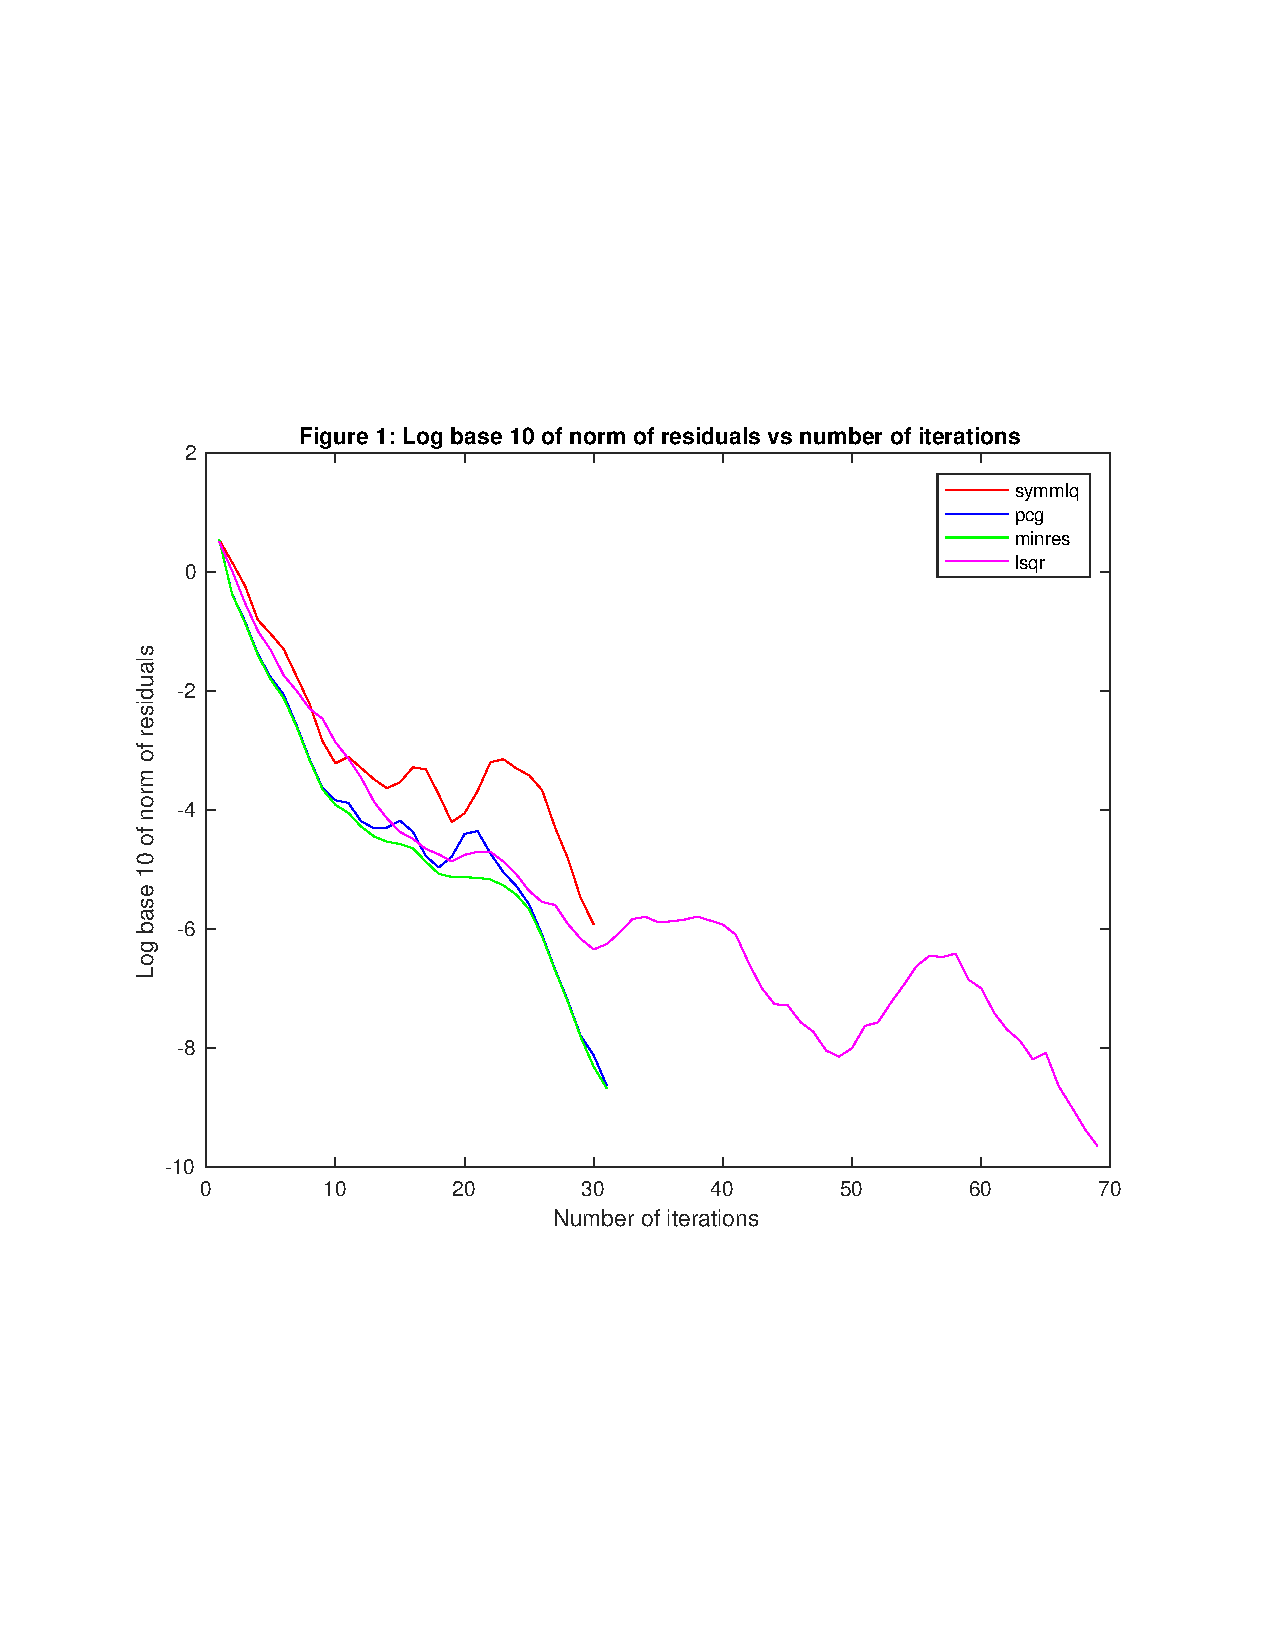
\includegraphics[scale=0.3]{fig1}
\captionof{figure}{Log base 10 norm of residuals over $k$ iterations.}
\label{fig:4solvers}
\end{center}
\end{figure}

\medskip

\begin{figure}[H]
\begin{center}
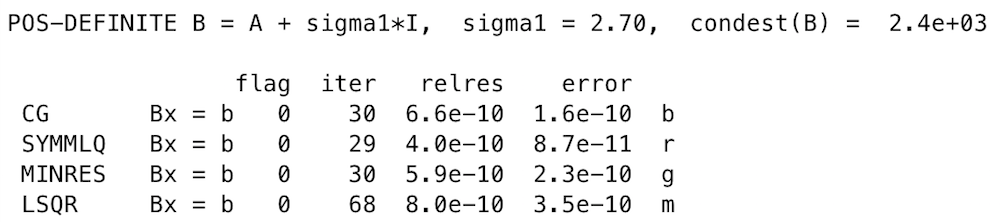
\includegraphics[scale=0.7]{fig2}
\captionof{figure}{A comparison between 4 solvers in terms of total iterations, relative residuals, and the error term at convergence.}
\label{fig:4solvers_table}
\end{center}
\end{figure}

\item[(b)]  All four solvers (PCG, MINRES, SYMMLQ, and LSQR) converged within a specified tolerance set to  1e-9 and hence their relative residuals in Figure  \ref{fig:4solvers_table} are on the same order of magnitude (order of 1e-10). In terms of log base 10 norm of residuals,  $\norm{r_k}$ , we notice that LSQR performs the best while SYMMLQ performs the worst. The difference between these two methods is approximately four orders of magnitude, which is significant. In terms of the number of iterations needed to reach the convergence, solvers PCG, MINRES, and SYMMLQ used 29-30 iterations while LSQR needed 68 iterations (almost twice as much). There are a couple of properties we can check on $A$ and $B$ in order to explain these differences:

\begin{enumerate}
\item[(i)]  $A$ is symmetric (checked by \verb|issymmetric(A)|), which favors PCG, MINRES, and SYMMLQ solvers in terms of the number of iterations since they work well for symmetric  case $Ax = b$. LSQR is typically applied on unsymmetric square or rectangular $A$.
\item[(ii)]  $A$ is ill-conditioned since its condition number is 1.1441e+07. This situation favors LSQR, which is consistent with Question 3 where  $C$ is also ill-conditioned and LSQR performs the best.
\item[(iii)]  $B$ is reasonably well-conditioned since its condition number is 2353. Therefore small differences between 3 solvers (PCG, MINRES, and SYMMLQ) should not be affected by cond($B$).
\end{enumerate}

Generally, it is reasonable to expect that PCG, MINRES, and SYMMLQ converge to the specified tolerance within roughly the same number of iterations. All four solvers seek to minimize $\norm{r_k}$ where $r_k = V_{k+1} t_{k+1}$ and $t_{k+1} \equiv \beta_1 e_1 - H_k y_k$. Specifically, PCG, MINRES, and SYMMLQ utilize Lanczos process while LSQR utilizes Golub-Kahan process. Therefore, each solver deals with a different subproblem:


\begin{enumerate}
\item[(i)]  CG: makes $t_{k+1} = 0$ everywhere except its last element 
\item[(ii)] MINRES: minimizes $\norm{r_k}$ such that $x_k = Vk y_k$
\item[(iii)] SYMMLQ: makes $t_{k+1} = 0$ everywhere except its last two elements while keeping $\norm{y_k}$ as small as possible
\item[(iv)] LSQR: similar as MINRES,  minimizes $\norm{r_k}$ such that $x_k = Vk y_k$
\end{enumerate}

\medskip 

\item[(c)]  The following stopping rules are implemented:

\begin{enumerate}
\item[(i)] PCG: uses the condition \texttt{(normr <= tolb || stag >= maxstagsteps || moresteps)}, where \texttt{normr} = $\norm{r_k}$, \texttt{tolb = tol} $\norm{b}$,  \texttt{maxstagsteps} is set to 3 and refers to a stagnation where two consecutive iterations produce roughly the same results, and \texttt{moresteps} is an indicator for exceeding the maximum number of steps.
\item[(ii)] MINRES: uses the condition \texttt{(normr <= tolb || stag >= maxstagsteps || moresteps)}, with parameters being the same as above.
\item[(iii)] SYMMLQ: uses the condition \texttt{(normr <= tolb || stag >= maxstagsteps || moresteps)}, with parameters being the same as above.
\item[(iii)] LSQR: uses the condition \texttt{(normr <= tolb)}, with parameters being the same as above. Additionally, LSQR checks for convergence in $min\; {|b-Ax|}$
\end{enumerate}


As a result, PCG, MINRES, and SYMMLQ use the same stopping criteria consisting of $\norm{r_k}$ being below some treshold, number of iterations not exceeding the maximum limit, and stagnation not exceeding 3 steps. LSQR also utilizes $\norm{r_k}$ being below some treshold and considers convergence in $min\; {|b-Ax|}$. This explains why PCG, MINRES, and SYMMLQ used roughly the same number of iterations whereas the additional criterion in LSQR might have led to additional iterations with better performance.

\end{itemize}



\item 
\begin{itemize}
\item[(a)]  Figure \ref{fig:4solvers_case2} compares the log base 10 norm of residuals $\norm{r_k}$ for each iteration $k$ for case when $Cx = b$ with $C$ being indefinite. Additionally, Figure \ref{fig:4solvers_table_case2} summarizes the results in terms of number of total iterations, relative residuals, and error term.

\begin{figure}[H]
\begin{center}
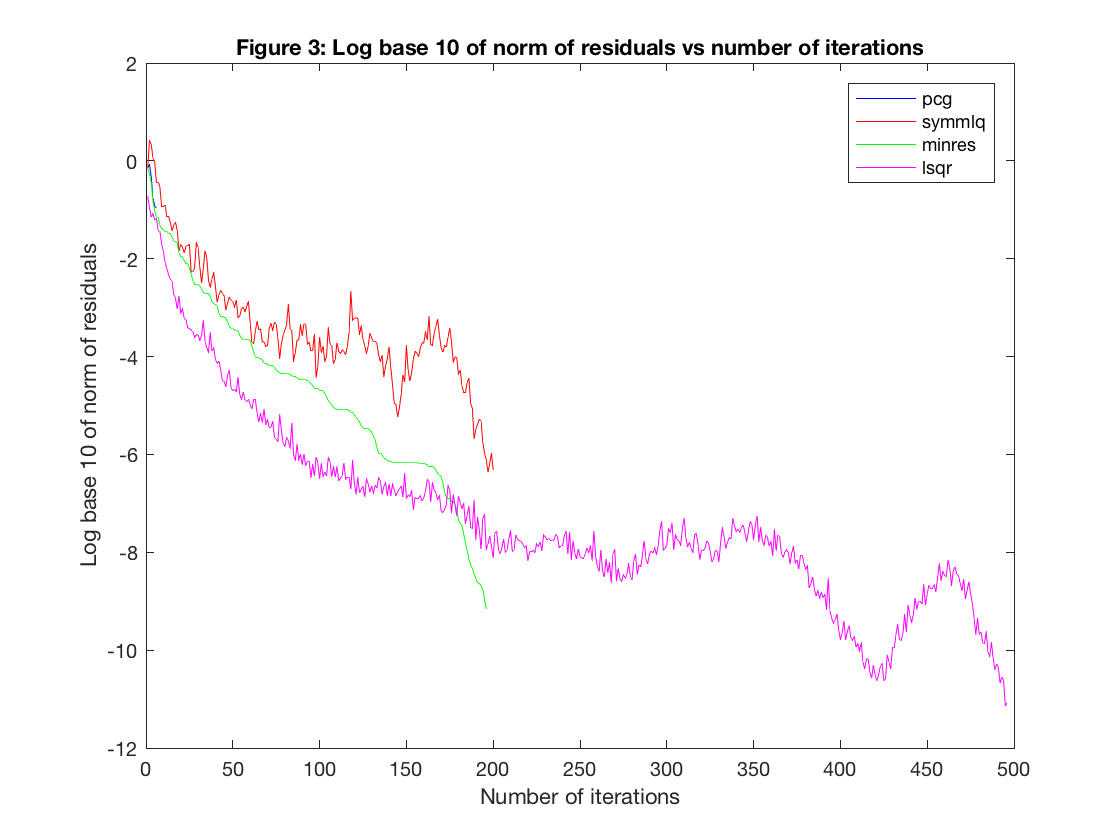
\includegraphics[scale=0.3]{fig3}
\captionof{figure}{Log base 10 norm of residuals over $k$ iterations for case $Cx = b$.}
\label{fig:4solvers_case2}
\end{center}
\end{figure}

\medskip

\begin{figure}[H]
\begin{center}
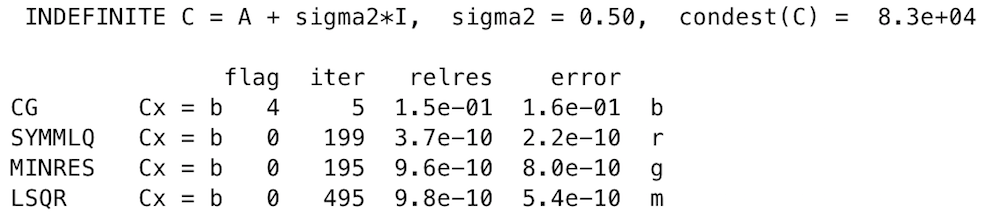
\includegraphics[scale=0.7]{fig4}
\captionof{figure}{A comparison between 4 solvers in terms of total iterations, relative residuals, and the error term at convergence for case $Cx = b$.}
\label{fig:4solvers_table_case2}
\end{center}
\end{figure}

\medskip

\item[(b)] Since $C$ is not a positive-definite matrix, the PCG solver terminated after 5 iterations. In Figure \ref{fig:4solvers_table_case2}, we see that \texttt{flag = 4} is being raised to explain the early stopping. The flag refers to the condition when \texttt{one of the scalar quantities calculated during PCG became too small or too large to continue computing}. Hence the solver stopped the process once it was realized that $C$ is ill-conditioned. In situations when $C$ is positive-definite, each $T_k$ is theoretically positive-definite and PCG can obtain Cholesky factors $T_k = L_k D_k {T_k}^T$. In situations when $C$ is not positive-definite, some $T_k$ may be singular but $T_k$ cannot be singular twice in a row. In this case, it was probably the second scenario leading to the breakdown.

\item[(c)] Consistent with the problem setup in Question 2, here $C$ is also ill-conditioned (its condition number is 8.2837e+04). Similarly, LSQR performs the best and SYMMLQ performs the worst. The difference between the two methods is approximately 5 orders of magnitude, which is significant. In terms of the number of iterations to reach the convergence, MINRES and SYMMLQ utilized roughly the same number of iterations (195 and 199). This is expected due to the same convergence criteria summarized in Question 2. Again LSQR needs more than twice the number of iterations to reach the convergence but leads to a better performance since the system is ill-conditioned.
\end{itemize}

\medskip

\item Figures \ref{fig:distr1} and \ref{fig:distr2} show the distribution of eigenvalues for case $Cx = b$. $\lambda(C)$ lie on the interval [-2.1830, 7.3331], however, some of them are repeated -- for instance, $\lambda(C)$ = 0.5032 is repeated three times. Additionally, from Figure \ref{fig:distr2} we can deduce that a significant majority of eigenvalues are concentrated on the interval [0.5, 0.6]. More precisely, roughly 280 eigenvalues are concentrated around the value of 0.5. The repeated values of $\lambda(C)$ suggest that C could be viewed as a matrix with fewer than $n$ distinct eigenvalues either because some of them repeated or some of them are very similar to each other to the extent of being regarded as essentially the same. In previous problem set, we established that if $A$ has $m < n$ distinct eigenvalues, the Lanczos process will use at most $m$ iterations. Similarly, in our case the number of distinct eigenvalues is also less than $n$, and hence the solvers would require significantly fewer than $n$ iterations.
 
\begin{figure}[H]
\begin{center}
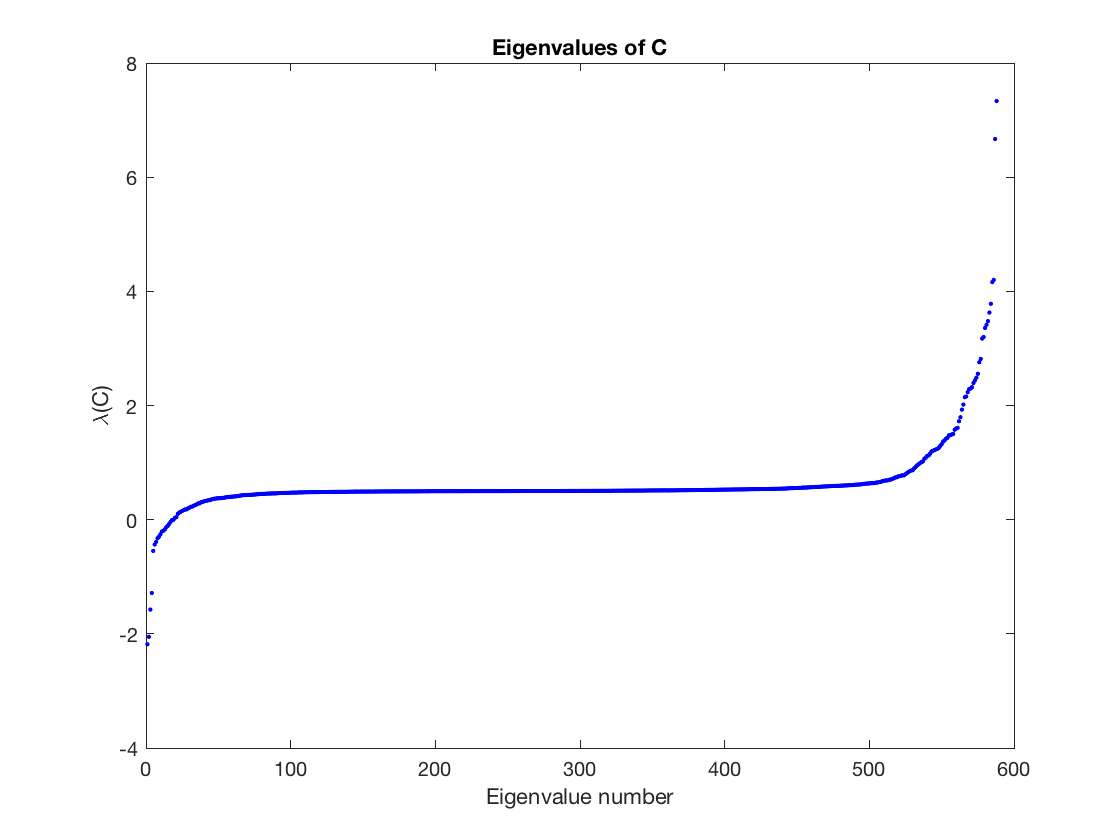
\includegraphics[scale=0.3]{fig5}
\captionof{figure}{Distribution of eigenvalues for case $Cx = b$..}
\label{fig:distr1}
\end{center}
\end{figure}

\medskip

\begin{figure}[H]
\begin{center}
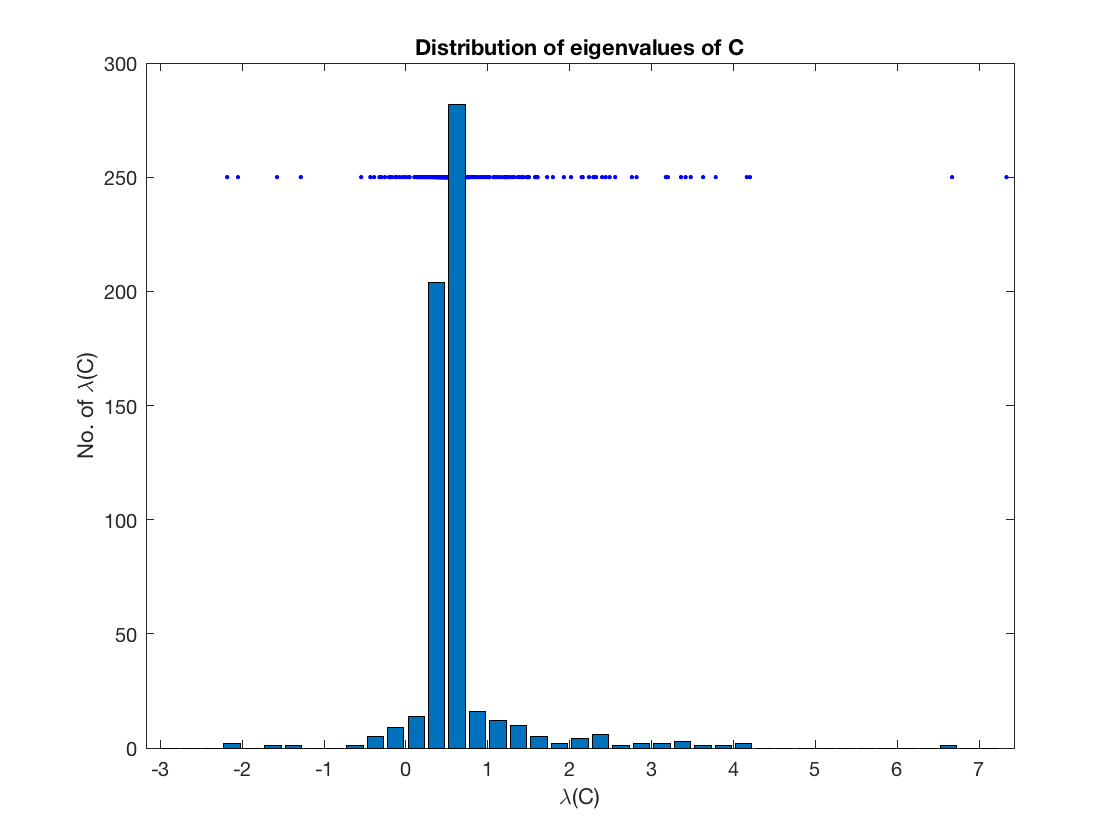
\includegraphics[scale=0.3]{fig6}
\captionof{figure}{Distribution of eigenvalues for case $Cx = b$.}
\label{fig:distr2}
\end{center}
\end{figure}

\medskip

\begin{figure}[H]
\begin{center}
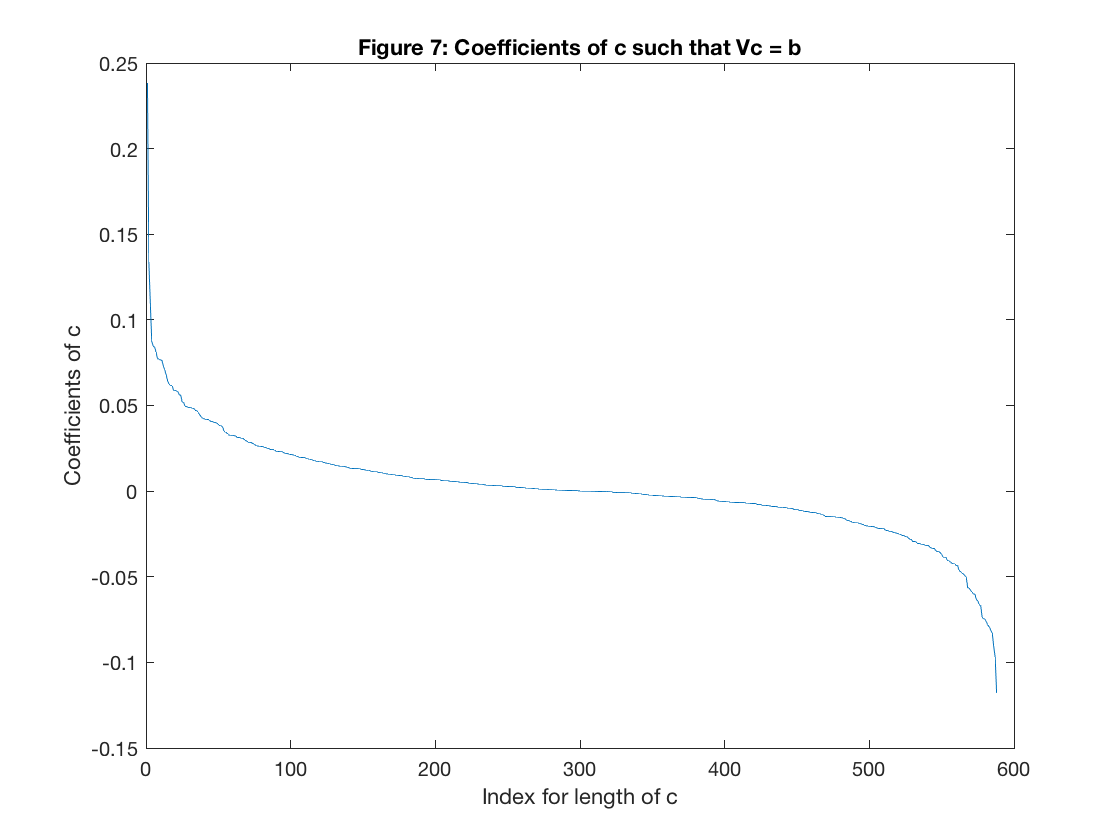
\includegraphics[scale=0.3]{fig7}
\captionof{figure}{Coefficients of c such that $Vc = b$.}
\label{fig:c}
\end{center}
\end{figure}

We can also obtain the full eigendecomposition of $C$ and write the relationship $Vc = b$, where $V$ represents an orthogonal matrix whose columns are corresponding eigenvectors of $C$ and $c$ represents a vector whose coefficients satisfy the following equalities:

\begin{enumerate}
\item[(i)] $Vc = b$
\item[(ii)] $c = V^T b$
\end{enumerate}

Hence, $c$ is coefficient vector, which represents $b$ in terms of the eigenvector basis of $C$. Figure \ref{fig:c} reveals that a majority of coefficients are near-zero values though they never actually become zero. Therefore, it may be plausible that the Lanczos process discards some of these near-zero coefficient eigenvectors, leading to an additional reduction in the number of iterations necessary to solve $Cx = b$. 

In conclusion, the combination of repeated or near-equivalent eigenvalues of $C$ and near-zero coefficients for eigenvectors of $C$ could explain why the symmetric solvers require significantly fewer than $n$ iterations.

Please find the code used to produce the graphs below.  


\end{enumerate}
\newpage

\begin{small}
\begin{verbatim}
% CGtest8.m is a script for comparing {cg, symmlq, minres}
% on sparse matrix Boeing/bcsstm34, n=588, nnz=24270).
% See http://faculty.cse.tamu.edu/davis/welcome.html (Tim Davis).
% The matrix A is from a structural problem.
% It is symmetric indefinite with lambda_min = -2.6830.
%
% 09 Apr 2017: Problem Boeing/bcsstm34 used for Homework 3.
% 22 Apr 2018: Removed pcg and minres on C^2x = Cb.
%----------------------------------------------------------

load bcsstm34.mat;   % lambda(min) = -2.6830, lambda(max) = 6.8331
A     = Problem.A;   % Save original matrix A
condest(A)
[n,n] = size(A);
x     = 1./(1:n)';

%----------------------------------------------------------
sigma1 = 2.7;
B      = A + sigma1*speye(n);   condB = condest(B);
b      = B*x;
tol    = 1e-9;   % Not highly accurate
maxit  = 1000;

[xC,flagC,relresC,iterC,resvecC]       = pcg   (B,b,tol,maxit);
[xL,flagL,relresL,iterL,resvecL]       = symmlq(B,b,tol,maxit);
[xM,flagM,relresM,iterM,resvecM]       = minres(B,b,tol,maxit);
[xS,flagS,relresS,iterS,resvecS,lsvec] = lsqr  (B,b,tol,maxit);

errC  = norm(xC-x,inf);   % The inf-norm is best for large vectors
errL  = norm(xL-x,inf);
errM  = norm(xM-x,inf);
errS  = norm(xS-x,inf);

fprintf('\nPOS-DEFINITE B = A + sigma1*I,')
fprintf('  sigma1 =%5.2f,  condest(B) = %8.1e\n\n', sigma1, condB)
fprintf('                flag  iter   relres    error\n')
fprintf(' CG       Bx = b%4g %5g %8.1e %8.1e  b\n', flagC,iterC,relresC,errC)
fprintf(' SYMMLQ   Bx = b%4g %5g %8.1e %8.1e  r\n', flagL,iterL,relresL,errL)
fprintf(' MINRES   Bx = b%4g %5g %8.1e %8.1e  g\n', flagM,iterM,relresM,errM)
fprintf(' LSQR     Bx = b%4g %5g %8.1e %8.1e  m\n', flagS,iterS,relresS,errS)

figure(1)
hold off;  plot(log10(resvecL),'r-')
hold  on;  plot(log10(resvecC),'b-')
hold  on;  plot(log10(resvecM),'g-')
hold  on;  plot(log10(lsvec)  ,'m-')
xlabel('Number of iterations') % x-axis label
ylabel('Log base 10 of norm of residuals') % y-axis label
legend('symmlq','pcg', 'minres', 'lsqr')
title('Figure 1: Log base 10 of norm of residuals vs number of iterations')

%----------------------------------------------------------
sigma2 = 0.5;
C      = A + sigma2*speye(n);   condC  = condest(C);
b      = C*x;    Cfun  = @(x) C*x;       % Treat  C  as a function
%b2    = C*b;    Cfun2 = @(x) C*(C*x);   % Treat C*C as a function

[xC,flagC,relresC,iterC,resvecC]       = pcg   (Cfun ,b ,tol,maxit);
[xL,flagL,relresL,iterL,resvecL]       = symmlq(Cfun ,b, tol,maxit);
[xM,flagM,relresM,iterM,resvecM]       = minres(Cfun ,b ,tol,maxit);
[xS,flagS,relresS,iterS,resvecS,lsvec] = lsqr  (C    ,b ,tol,maxit);

errC  = norm(xC-x,inf);
errL  = norm(xL-x,inf);
errM  = norm(xM-x,inf);
errS  = norm(xS-x,inf);

fprintf('\n  INDEFINITE C = A + sigma2*I,')
fprintf('  sigma2 =%5.2f,  condest(C) = %8.1e\n\n', sigma2, condC)
fprintf('                flag  iter   relres    error\n')
fprintf(' CG       Cx = b%4g %5g %8.1e %8.1e  b\n', flagC,iterC,relresC,errC)
fprintf(' SYMMLQ   Cx = b%4g %5g %8.1e %8.1e  r\n', flagL,iterL,relresL,errL)
fprintf(' MINRES   Cx = b%4g %5g %8.1e %8.1e  g\n', flagM,iterM,relresM,errM)
fprintf(' LSQR     Cx = b%4g %5g %8.1e %8.1e  m\n', flagS,iterS,relresS,errS)

figure(2)
hold off;  plot(log10(resvecC),'b-')
hold  on;  plot(log10(resvecL),'r-')
hold  on;  plot(log10(resvecM),'g-')
hold  on;  plot(log10(lsvec)  ,'m-')

xlabel('Number of iterations') % x-axis label
ylabel('Log base 10 of norm of residuals') % y-axis label
legend('pcg', 'symmlq', 'minres', 'lsqr')
title('Figure 3: Log base 10 of norm of residuals vs number of iterations')

%----------------------------------------------------------
% Plot the eigenvalues of C.
%----------------------------------------------------------
lambda = eig(full(C));
figure(3)
hold off;    plot(lambda,'b.')
xlabel('Eigenvalue number');   ylabel('\lambda(C)');
title('Eigenvalues of C');

% Show if the eigenvalues are clustered.
figure(4)
hold off;    plot(lambda,250*ones(n,1),'b.')
hold on

y1    = -3;      yn    =  7;
step  =  0.25;   nbar  = (yn - y1)/step + 1;
y     = zeros(nbar,1);
nlam  = zeros(nbar,1);

for i = 1:nbar
  y2      = y1 + step;
  nlam(i) = length( find(lambda>y1 & lambda<=y2) );
  y(i)    = y1 + 0.5*step;
  y1      = y2;
end

bar( y, nlam )
xlabel('\lambda(C)');   ylabel('No. of \lambda(C)');
title('Distribution of eigenvalues of C');

[V, D] = eig(full(C));
c = V\b;
figure(5)
plot(sort(c, 1, 'descend'))
xlabel('Index for length of c') % x-axis label
ylabel('Coefficients of c') % y-axis label
title('Figure 7: Coefficients of c such that Vc = b')



\end{verbatim}
\end{small}

\end{document}
